%% Overleaf version: compiles on its own (pdfLaTeX, no BibTeX). GENERATED by manuscript/make_overleaf.py
\documentclass[11pt]{article}
\usepackage[T1]{fontenc}
\usepackage[margin=2.3cm]{geometry}
\usepackage{amsmath}
\usepackage{amssymb}
\usepackage{booktabs}
\usepackage{graphicx}
\usepackage{float}
\usepackage{placeins}
\usepackage{xcolor}
\usepackage{listings}
\usepackage[colorlinks=true,linkcolor=blue,citecolor=blue,urlcolor=blue]{hyperref}
\setcounter{secnumdepth}{2}
\emergencystretch=2em
\renewcommand{\theequation}{N\arabic{equation}}
\renewcommand{\thetable}{N\arabic{table}}
\renewcommand{\thefigure}{N\arabic{figure}}
\renewcommand{\lstlistingname}{Code}

% print-safe Python style (same palette as the aniGTO manuscript)
\definecolor{codeBg}{RGB}{246,248,250}\definecolor{codeBorder}{RGB}{208,215,222}
\definecolor{codeKw}{RGB}{0,92,197}\definecolor{codeStr}{RGB}{154,68,0}
\definecolor{codeCom}{RGB}{31,122,72}\definecolor{codeNum}{RGB}{87,96,106}
\lstdefinestyle{py}{language=Python,basicstyle=\ttfamily\footnotesize,keywordstyle=\color{codeKw}\bfseries,
  stringstyle=\color{codeStr},commentstyle=\color{codeCom}\itshape,numbers=left,numberstyle=\tiny\color{codeNum},
  numbersep=6pt,backgroundcolor=\color{codeBg},frame=single,rulecolor=\color{codeBorder},framesep=3pt,
  xleftmargin=14pt,breaklines=true,breakatwhitespace=false,postbreak=\mbox{\textcolor{codeNum}{$\hookrightarrow$}\space},
  columns=fullflexible,keepspaces=true,showstringspaces=false,upquote=true,captionpos=t,
  literate={≥}{{$\ge$}}1 {≤}{{$\le$}}1 {−}{{-}}1}
\lstset{style=py}

% Reviewer support document.  Every number comes from files written by ../codes/04_exact_vs_proposed.py
% (results/iee_robust.csv, results/tab_exact_vs_proposed.tex, figures/dcscan_exact_vs_proposed.pdf); the code
% listings snip_*.py are copied verbatim from ../codes by make_eri_snippets.py.  Build with ./build.sh.

\title{Supporting document for reviewers:\\[4pt]
\Large Exact aniGTO electron-repulsion integrals at extreme anisotropy\\
by the logarithmic variable $s=\ln u$ in the Boys-type integral}
\author{Gabriel Chirchir, Subrata Jana, Szymon \'Smiga\\[2pt]
\small Institute of Physics, Nicolaus Copernicus University in Toru\'n, Poland}
\date{Companion to the manuscript ``Probing Dimensional Crossover in SCAN Exchange with Exact\\
Quasi-One-Dimensional Wires and Quasi-Two-Dimensional Sheets'' and its Supporting Information}

% Figures: names are unique to this paper (scan1d2d_*.pdf). Overleaf compiles from the project root, so if
% this folder sits inside a larger Overleaf project under a name not listed here, add {<folder>/figures/}.
\graphicspath{{figures/}{overleaf/figures/}{scan/figures/}{SCAN_1D_2D/figures/}{scan_1d_2d/figures/}{dcscan/figures/}{DC-SCAN/figures/}{scan1d2d/figures/}}
\begin{document}
\maketitle

\noindent\fcolorbox{black!40}{black!3}{\parbox{\dimexpr\linewidth-2\fboxsep-2\fboxrule}{%
\textbf{What is new, in four points.}
\begin{enumerate}\itemsep0pt
\item \emph{Problem.} aniGTO evaluates every anisotropic two-electron repulsion integral (ERI) as one
  Boys-type integral over $t=u/\sqrt{1+u^2}\in[0,1)$ (eq~\ref{n:eri-t}).  An exponent ratio $\rho$ puts its
  contribution at $1-t\approx1/(2\rho)$: it is under-resolved from $\rho\sim10^{8}$, and beyond
  $u^2=2^{52}\approx4.5\times10^{15}$ no double-precision $t<1$ exists at all.  The default routine then
  fails by up to 11.3~Ha (Table~\ref{n:tab}).
\item \emph{What we solved.} The same integral is rewritten in the scale-free variable $s=\ln u$
  (eq~\ref{n:logvar} = main-text eq~\href{main.pdf\#equation.1}{1}).  The closed-form aniGTO kernels $I_k$
  (eq~\ref{n:Ik-closed}, derived step by step in Section~\ref{n:sec:anigto}) are unchanged; we add explicit
  truncation bounds and an analytic small-$u$ piece (Section~\ref{n:sec:proposed}).
\item \emph{Proof of accuracy.} On the exactly solvable self-repulsion of anisotropic Gaussians (closed forms,
  main eqs~\href{main.pdf\#equation.10}{A10} and \href{main.pdf\#equation.11}{A11}) the error is $<10^{-11}$~mHa, the double-precision
  limit, for wire and sheet at every $\lambda=10^{1}$--$10^{8}$, i.e.\ exponent ratios up to $10^{16}$
  (Table~\ref{n:tab}, Figure~\ref{n:fig}).
\item \emph{Hamiltonian and code.} The orbitals are exact eigenfunctions of the one-particle trap Hamiltonian,
  solved analytically; no Kohn--Sham equation is solved (Section~\ref{n:sec:hamiltonian}).  All code is in
  \texttt{SCAN\_1D\_2D/codes/01--09}; the ERI is in \texttt{04\_exact\_vs\_proposed.py}, listed in
  Codes~\ref{n:code:kernel}--\ref{n:code:test} (Section~\ref{n:sec:codes}).
\end{enumerate}}}

\tableofcontents

%======================================================================================================
\section{The one-particle Hamiltonian: where the orbitals come from}
\label{n:sec:hamiltonian}
No Kohn--Sham (or Hartree--Fock) equation is solved self-consistently anywhere in this work, and no
script calls an SCF solver.  All results are \emph{fixed-density, exchange-only}: exchange functionals are
evaluated on densities whose orbitals are known exactly.  Those orbitals are the eigenfunctions of the
one-particle anisotropic harmonic-trap Hamiltonian
\begin{equation}
\hat h=-\tfrac12\nabla^2+\tfrac12\sum_{k=x,y,z}\omega_k^2x_k^2 ,
\label{n:h}
\end{equation}
which separates into three one-dimensional oscillators and is solved \emph{analytically}:
\begin{equation}
\hat h\,\phi_{\mathbf n}=\varepsilon_{\mathbf n}\phi_{\mathbf n},\qquad
\phi_{\mathbf n}(\mathbf r)=\prod_k\omega_k^{1/4}\,h_{n_k}\!\bigl(\sqrt{\omega_k}\,x_k\bigr),\qquad
\varepsilon_{\mathbf n}=\sum_k\omega_k\bigl(n_k+\tfrac12\bigr),
\label{n:h-eig}
\end{equation}
with the Hermite functions $h_n$ of SI eq~\href{si.pdf\#equation.4}{S4}.  The ground state is the normalized aniGTO
$s$ function of the harmonic-trap (``dot'') basis, with exponents $\alpha_k=\omega_k/2$ (SI
eqs~\href{si.pdf\#equation.1}{S1}--\href{si.pdf\#equation.3}{S3}):
\begin{equation}
\phi_{\mathbf 0}(\mathbf r)=\prod_k\Bigl(\frac{\omega_k}{\pi}\Bigr)^{1/4}e^{-\omega_kx_k^2/2},\qquad
n(\mathbf r)=2\phi_{\mathbf 0}^2,
\label{n:density}
\end{equation}
which is the reference density of the manuscript: $\boldsymbol\omega=(1,1,\lambda^2)$ for the sheet and
$(\lambda^2,\lambda^2,1)$ for the wire (main eqs~\href{main.pdf\#equation.7}{A7} and \href{main.pdf\#equation.8}{A8}).  For $N=2$ (one
doubly occupied orbital) the exact exchange energy is a single ERI (main eq~\href{main.pdf\#equation.9}{A9}),
\begin{equation}
E_x=-\tfrac12E_H=-(\phi_{\mathbf 0}\phi_{\mathbf 0}|\phi_{\mathbf 0}\phi_{\mathbf 0}),
\label{n:ex}
\end{equation}
which is why the accuracy of that one integral decides the benchmark.  The $N=4$ and 6 wires of the SI occupy
the $s$, $p_z$, $d_{zz}$ eigenfunctions ($n_z=0,1,2$) of the same $\hat h$.  Because $\hat h$ is solved in
closed form there is no basis-set or SCF error in any reference.  The self-consistent potential of DC-SCAN is
derived in main Appendix~\href{main.pdf\#subsection.A.9}{A.9} but is not used here: self-consistent runs are future work.

Code~\ref{n:code:trap} shows how script \texttt{03} builds this orbital (class \texttt{TrapS}, with
exponents $\omega_k/2$ and normalization $\prod_k(2\alpha_k/\pi)^{1/4}$), takes the exact exchange from the aniGTO ERI
(\texttt{build\_wire}), and forms $n$, $\nabla n$, $\nabla\nabla n$ and $\tau$ from the analytic derivatives
(\texttt{density\_fields}; SI eqs~\href{si.pdf\#equation.16}{S16} and \href{si.pdf\#equation.17}{S17}).  PySCF enters only through
\texttt{eval\_xc}, which evaluates libxc exchange functionals on these fields.

\begin{lstlisting}[caption={The analytic trap orbital and its density fields (script \texttt{03}, verbatim).},label=n:code:trap]
# codes/03_anigto_wire_libxc.py (verbatim)

class TrapS:
    """The s function of the aniGTO harmonic-trap ('dot') basis for omega = (wx, wy, wz): a normalized anisotropic
    Gaussian with exponents omega/2, i.e. phi(r) = prod_k (omega_k/pi)^(1/4) exp(-omega_k x_k^2 / 2).
    Attributes follow the aniGTO BasisFunction object (exps, shell, origin, coefs, norm, num_coefs)."""

    def __init__(self, omega):
        a = 0.5 * np.asarray(omega, dtype=float)
        self.exps = a.reshape(1, 3)
        self.shell = (0, 0, 0)
        self.origin = (0.0, 0.0, 0.0)
        self.coefs = np.array([1.0])
        self.norm = np.array([np.prod((2.0 * a / np.pi) ** 0.25)])
        self.num_coefs = 1

class TrapMolecule:
    """Minimal stand-in for aniGTO Molecule(basis='dot', n_orbitals={'S': 1}): one trap s function."""

    def __init__(self, omega):
        self.bfs = [TrapS(omega)]

def build_wire(lam, workdir=None):
    """Wire trap omega = (lam^2, lam^2, 1); returns (molecule, exact E_x = -(phi phi|phi phi) from aniGTO IEE)."""
    mol = TrapMolecule([lam ** 2, lam ** 2, 1.0])
    b = mol.bfs[0]
    a, L, O = tuple(b.exps[0]), (0, 0, 0), (0.0, 0.0, 0.0)
    with warnings.catch_warnings():
        warnings.simplefilter('ignore')
        eri = b.norm[0] ** 4 * IEE(a, L, O, a, L, O, a, L, O, a, L, O)
    assert np.allclose(b.exps[0], [lam ** 2 / 2, lam ** 2 / 2, 0.5]), b.exps
    return mol, -eri

def density_fields(mol, coords):
    """rho, grad rho, Hessian of rho, laplacian, tau for the doubly occupied aniGTO s orbital."""
    phi, g, h = eval_bf_hess(mol.bfs[0], coords)
    rho = 2.0 * phi * phi
    grad = 4.0 * phi * g
    hess = 4.0 * (g[:, None, :] * g[None, :, :] + phi * h)
    lap = np.trace(hess)
    tau = np.sum(g * g, axis=0)                          # 1/2 sum_occ f |grad phi|^2 with f = 2
    return rho, grad, hess, lap, tau
\end{lstlisting}

%======================================================================================================
\section{Derivation of the aniGTO repulsion integral}
\label{n:sec:anigto}
The derivation follows the aniGTO notes (SI Section~\href{si.pdf\#section.1}{S1}) and uses only three
tools.  Each step names the code line that implements it (Code~\ref{n:code:kernel}).

\subsection{Tools and notation}
\paragraph{Gaussian product theorem.}
\begin{equation}
e^{-\alpha(x-A)^2}e^{-\beta(x-B)^2}=E_{AB}\,e^{-(\alpha+\beta)(x-P)^2},\qquad
P=\frac{\alpha A+\beta B}{\alpha+\beta},\qquad E_{AB}=e^{-\frac{\alpha\beta}{\alpha+\beta}(A-B)^2}.
\label{n:gpt}
\end{equation}
\paragraph{Binomial theorem.}
\begin{equation}
(x+a)^n=\sum_{i=0}^{n}\binom{n}{i}x^ia^{n-i},
\label{n:binom}
\end{equation}
applied factor by factor to products $(x+a)^n(x+b)^m\cdots$.
\paragraph{Gaussian moments} (\texttt{integral(a,b)} with \texttt{fact2}):
\begin{equation}
\int_{-\infty}^{+\infty}x^ne^{-\alpha x^2}dx=\sqrt{\frac{\pi}{\alpha}}\,\frac{(n-1)!!}{(2\alpha)^{n/2}}
\quad(n\ \text{even}),\qquad 0\quad(n\ \text{odd}),\qquad(-1)!!=1 .
\label{n:moment}
\end{equation}
Combining eqs~\ref{n:binom} and \ref{n:moment}, a product of four shifted monomials under one Gaussian
centred at $U$ is (\texttt{integral2(alpha,U,a,A,b,B,c,C,d,D)})
\begin{equation}
\int\prod_{i=1}^{4}(x-X_i)^{n_i}e^{-\beta(x-U)^2}dx
=\sum_{j_1\ldots j_4}\prod_{i=1}^4\binom{n_i}{j_i}(U-X_i)^{n_i-j_i}
\sqrt{\frac{\pi}{\beta}}\frac{(J-1)!!}{(2\beta)^{J/2}},\quad J=\textstyle\sum_ij_i\ \text{even}.
\label{n:int2}
\end{equation}
\paragraph{Anisotropic Gaussians.}  A primitive has one exponent and one power per axis,
\begin{equation}
G_A(\mathbf r,\boldsymbol\alpha,\mathbf n,\mathbf A)=\prod_{k=x,y,z}(x_k-A_k)^{n_k}e^{-\alpha_k(x_k-A_k)^2}.
\label{n:prim}
\end{equation}

\subsection{The two-electron repulsion integral and its factorization}
\begin{equation}
I^{EE}_{ABCD}=\iint d\mathbf r_1d\mathbf r_2\,
\frac{G_A(\mathbf r_1,\boldsymbol\alpha,\mathbf n,\mathbf A)\,G_B(\mathbf r_1,\boldsymbol\beta,\mathbf m,\mathbf B)\,
G_C(\mathbf r_2,\boldsymbol\gamma,\mathbf p,\mathbf C)\,G_D(\mathbf r_2,\boldsymbol\delta,\mathbf q,\mathbf D)}{r_{12}} .
\label{n:eri-def}
\end{equation}
The Laplace (Gaussian) transform of the Coulomb operator (SI eq~\href{si.pdf\#equation.8}{S8}),
\begin{equation}
\frac1{r_{12}}=\frac{2}{\sqrt\pi}\int_0^\infty e^{-u^2r_{12}^2}\,du,\qquad
r_{12}^2=\sum_k(x_{1k}-x_{2k})^2,
\label{n:coulomb}
\end{equation}
turns $1/r_{12}$ into a product over axes.  With eq~\ref{n:gpt} for the pairs $(A,B)$ on electron 1 and
$(C,D)$ on electron 2 the six-dimensional integral factorizes for every $u$:
\begin{equation}
I^{EE}_{ABCD}=\frac{2}{\sqrt\pi}\,E\int_0^\infty du\,I_x(u^2)\,I_y(u^2)\,I_z(u^2),\qquad
E=\prod_kE_{k,AB}E_{k,CD},
\label{n:eri-u}
\end{equation}
\begin{multline}
I_x(u^2)=\iint dx_1dx_2\,(x_1-A)^{n}(x_1-B)^{m}(x_2-C)^{p}(x_2-D)^{q}\\
\times e^{-(\alpha+\beta)(x_1-P_{AB})^2}e^{-(\gamma+\delta)(x_2-P_{CD})^2}e^{-u^2(x_1-x_2)^2},
\label{n:Ix}
\end{multline}
where the axis label is dropped on $\alpha,\ldots,q$ and $A,\ldots,D$ (SI eqs~\href{si.pdf\#equation.9}{S9} and
\href{si.pdf\#equation.10}{S10}).  This is the structure of \texttt{IEE}: the prefactor $E$ (\texttt{ExAB}\ldots\texttt{EzCD})
times the $u$ integral of the product of three calls of \texttt{integral3}.

\subsection{The $x_1$ integral}
Completing the square in $x_1$,
\begin{equation}
\begin{gathered}
e^{-(\alpha+\beta)(x_1-P_{AB})^2-u^2(x_1-x_2)^2}=e^{-(\alpha+\beta+u^2)(x_1-Q)^2}\,e^{-\xi(x_2-P_{AB})^2},\\
Q=\frac{(\alpha+\beta)P_{AB}+u^2x_2}{\alpha+\beta+u^2},\qquad
\xi=\frac{(\alpha+\beta)u^2}{\alpha+\beta+u^2}
\end{gathered}
\label{n:x1}
\end{equation}
(\texttt{xi}, \texttt{PAB} in \texttt{integral3}).  Writing $x_1-A=(x_1-Q)+(Q-A)$, expanding binomially and using
eq~\ref{n:moment} for $x_1-Q$:
\begin{multline}
\int dx_1(x_1-A)^n(x_1-B)^me^{-(\alpha+\beta+u^2)(x_1-Q)^2}\\
=\sqrt{\frac{\pi}{\alpha+\beta+u^2}}\sum_{i,j}^{i+j\ \mathrm{even}}\binom ni\binom mj
\frac{(i+j-1)!!}{[2(\alpha+\beta+u^2)]^{(i+j)/2}}(Q-A)^{n-i}(Q-B)^{m-j}.
\label{n:x1-int}
\end{multline}
$Q$ depends on $x_2$; the shifted-centre identity
\begin{equation}
Q-A=\frac{u^2}{\alpha+\beta+u^2}\bigl(x_2-A'\bigr),\qquad
A'(u^2)=\frac{A(\alpha+\beta+u^2)-(\alpha+\beta)P_{AB}}{u^2}
\label{n:shift}
\end{equation}
(and likewise $B'$; \texttt{A1}, \texttt{B1} in \texttt{integral3}) makes the remaining $x_2$ integrand a
polynomial in $x_2$ times Gaussians.

\subsection{The $x_2$ integral and the closed form}
The two $x_2$ Gaussians combine by eq~\ref{n:gpt}:
\begin{equation}
\begin{gathered}
e^{-(\gamma+\delta)(x_2-P_{CD})^2}e^{-\xi(x_2-P_{AB})^2}
=e^{-\frac{(\gamma+\delta)\xi}{\gamma+\delta+\xi}(P_{CD}-P_{AB})^2}\,e^{-(\gamma+\delta+\xi)(x_2-U)^2},\\
U=\frac{(\gamma+\delta)P_{CD}+\xi P_{AB}}{\gamma+\delta+\xi}
\end{gathered}
\label{n:x2}
\end{equation}
(\texttt{U} and the exponential in \texttt{integral3}).  The $x_2$ integral is then eq~\ref{n:int2} with
$\beta=\gamma+\delta+\xi$ and the four factors $(x_2-C)^p(x_2-D)^q(x_2-A')^{n-i}(x_2-B')^{m-j}$
(\texttt{integral2(c+d+xi,U,n-i,A1,m-j,B1,p,C,q,D)}).  Collecting,
\begin{multline}
I_x(u^2)=\sqrt{\frac{\pi}{\alpha+\beta+u^2}}\sqrt{\frac{\pi}{\gamma+\delta+\xi}}\;
e^{-\frac{(\gamma+\delta)\xi}{\gamma+\delta+\xi}(P_{CD}-P_{AB})^2}\\
\times\sum_{i=0}^{n}\sum_{j=0}^{m}\binom ni\binom mj\frac{(i+j-1)!!}{[2(\alpha+\beta+u^2)]^{(i+j)/2}}
\Bigl(\frac{u^2}{\alpha+\beta+u^2}\Bigr)^{n+m-i-j}\\
\times\sum_{k=0}^{p}\sum_{l=0}^{q}\sum_{r=0}^{n-i}\sum_{s'=0}^{m-j}
\binom pk\binom ql\binom{n-i}{r}\binom{m-j}{s'}
\frac{(k+l+r+s'-1)!!}{[2(\gamma+\delta+\xi)]^{(k+l+r+s')/2}}\\
\times(U-C)^{p-k}(U-D)^{q-l}(U-A')^{n-i-r}(U-B')^{m-j-s'},
\label{n:Ik-closed}
\end{multline}
with only even $i+j$ and even $k+l+r+s'$ contributing (SI eq~\href{si.pdf\#equation.12}{S12}).
\emph{Eq~\ref{n:Ik-closed} is exact and closed-form in $u^2$}: no approximation has been made so far, and
the only numerical step left is the single $u$ integral of eq~\ref{n:eri-u}.

\subsection{Connection to the Boys function, and why anisotropy breaks it}
For an isotropic $s$-type quartet ($n=m=p=q=0$) with $p_{1}=\alpha+\beta$, $p_{2}=\gamma+\delta$ on every axis,
reduced exponent $\varrho=p_1p_2/(p_1+p_2)$ and $\mathbf R=\mathbf P_{AB}-\mathbf P_{CD}$, eq~\ref{n:Ik-closed}
has one term and $(p_1+u^2)(p_2+\xi)=(p_1+p_2)(\varrho+u^2)$, so
\begin{equation}
\prod_kI_k(u^2)=\frac{\pi^3}{(p_1+p_2)^{3/2}(\varrho+u^2)^{3/2}}\,
\exp\!\Bigl(-\frac{\varrho u^2}{\varrho+u^2}R^2\Bigr).
\label{n:iso}
\end{equation}
The Boys substitution $t_\varrho=u/\sqrt{\varrho+u^2}$, $dt_\varrho=\varrho(\varrho+u^2)^{-3/2}du$, removes the
scale exactly:
\begin{equation}
\int_0^\infty\prod_kI_k\,du=\frac{\pi^3}{(p_1+p_2)^{3/2}\varrho}\int_0^1e^{-Tt^2}dt
=\frac{\pi^3}{(p_1+p_2)^{3/2}\varrho}\,F_0(T),\qquad T=\varrho R^2,
\label{n:boys}
\end{equation}
which with eq~\ref{n:eri-u} is the familiar $(ss|ss)=2\pi^{5/2}E\,F_0(T)/(p_1p_2\sqrt{p_1+p_2})$ of
Boys~\cite{boys1950}; the integrand $e^{-Tt^2}$ is smooth on $[0,1]$ for any exponents.

For anisotropic primitives every axis has its own reduced exponent $\varrho_k$, and
$\prod_kI_k\propto\prod_k(\varrho_k+u^2)^{-1/2}\times(\ldots)$.  \emph{No single substitution removes three
different scales.}  aniGTO therefore uses the fixed scale $\varrho=1$, $t=u/\sqrt{1+u^2}$,
$u^2=t^2/(1-t^2)$, $du=(1-t^2)^{-3/2}dt$ (SI eq~\href{si.pdf\#equation.13}{S13}):
\begin{equation}
I^{EE}_{ABCD}=\frac{2}{\sqrt\pi}\,E\int_0^1\frac{dt}{(1-t^2)^{3/2}}\,
I_x\!\Bigl(\frac{t^2}{1-t^2}\Bigr)I_y\!\Bigl(\frac{t^2}{1-t^2}\Bigr)I_z\!\Bigl(\frac{t^2}{1-t^2}\Bigr),
\label{n:eri-t}
\end{equation}
evaluated by adaptive quadrature (\texttt{scipy.integrate.quad}, tolerances $10^{-16}$; \texttt{integrand2}
and \texttt{IEE}, Code~\ref{n:code:default}).  This is the ``aniGTO default'' baseline of Table~\ref{n:tab}.

%======================================================================================================
\section{Why the default $t$ quadrature fails at large anisotropy}
\label{n:sec:failure}
\paragraph{(i) Location.}  Axis $k$ changes the integrand where $u^2\sim\varrho_k$.  Since
$1-t=1-u/\sqrt{1+u^2}\simeq1/(2u^2)$ for $u\gg1$, an exponent scale $\varrho$ is mapped to
\begin{equation}
1-t\simeq\frac1{2\varrho}.
\label{n:loc}
\end{equation}
Exponent ratios $10^{8}$ and $10^{16}$ (wire $\lambda=10^4$ and $10^8$) put the feature at $1-t\sim10^{-8}$
and $10^{-16}$.

\paragraph{(ii) Shape: a near-singularity in $t$.}  For the wire self-repulsion
($A=2\boldsymbol\alpha=\mathrm{diag}(\lambda^2,\lambda^2,1)$, eq~\ref{n:self} below) the $u$ integrand is
$g(u)=\lambda^2/[(\lambda^2+2u^2)\sqrt{1+2u^2}]\simeq1/(\sqrt2\,u)$ for $1\ll u\ll\lambda$.  With
$1-t=\delta$, $u\simeq(2\delta)^{-1/2}$ and $du/dt=(1-t^2)^{-3/2}\simeq(2\delta)^{-3/2}$, the $t$ integrand is
\begin{equation}
g\,\frac{du}{dt}\simeq\frac{1}{2\sqrt2\,(1-t)},\qquad \frac1{\lambda^2}\lesssim1-t\ll1 ,
\label{n:tsing}
\end{equation}
a $1/(1-t)$ near-singularity cut off only at $1-t\sim\lambda^{-2}$.  It carries the whole wire logarithm,
$\int d\delta/(2\sqrt2\,\delta)=\ln\lambda/\sqrt2$, which after the prefactor $2/\sqrt\pi$ is the exact
$\sqrt{2/\pi}\ln\lambda$ of main eq~\href{main.pdf\#equation.13}{A13}.  An adaptive rule must resolve $\sim\ln\lambda^2$
decades of $1-t$ next to the endpoint.

\paragraph{(iii) Round-off and the end of double precision.}  The kernel argument $u^2=t^2/(1-t^2)$ is
computed from the difference $1-t^2$, whose relative round-off is $\epsilon/(1-t^2)\approx2\epsilon u^2$
($\epsilon=2^{-53}$): $\approx2\times10^{-6}$ relative error in $u^2$ at $u^2=10^{10}$.  The largest double below 1
is $t_{\max}=1-2^{-53}$, for which $u^2_{\max}=t_{\max}^2/(1-t_{\max}^2)=2^{52}-1\approx4.5\times10^{15}$: larger
$u$ cannot be represented in $t$ at all, while the wire at $\lambda=10^8$ needs $u^2$ up to
$\sim\lambda^2/2=5\times10^{15}$.

\paragraph{Observed consequence} (Table~\ref{n:tab}).  The default is exact to $3\times10^{-9}$~mHa up to
$\lambda=10^3$, loses 0.067~mHa (wire) and 0.080~mHa (sheet) at $\lambda=10^4$, and for $\lambda\ge10^5$ the wire
value freezes at $-3.906$~Ha (errors 5833 to 11344~mHa).  On the sheet the default returns
$-1.253314137=-\sqrt{\pi/2}$, the $\lambda\to\infty$ limit, for every $\lambda\ge10^5$: it misses exactly the
$\sqrt{2/\pi}\,\lambda^{-1}$ term that comes from $u\sim\lambda$ (error $8.0\times10^{-3}$~mHa at $10^5$, decreasing
as $\lambda^{-1}$).  The short wall times of the default at $\lambda\ge10^5$ (5~ms) are this failure, not a
speed-up.

%======================================================================================================
\section{The proposed method: the Boys-type integral in $s=\ln u$}
\label{n:sec:proposed}
\subsection{The equation that is solved}
Because $dt\,(1-t^2)^{-3/2}=du=e^s\,ds$, eq~\ref{n:eri-t} is identically
\begin{equation}
I^{EE}_{ABCD}=\frac{2}{\sqrt\pi}\,E\int_{-\infty}^{\infty}f(s)\,ds,\qquad
f(s)=e^{s}\,I_x\!\left(e^{2s}\right)I_y\!\left(e^{2s}\right)I_z\!\left(e^{2s}\right),\qquad s=\ln u,
\label{n:logvar}
\end{equation}
which is main-text eq~\href{main.pdf\#equation.1}{1}.  The aniGTO kernels are unchanged: $I_k$ is still the closed form
eq~\ref{n:Ik-closed} (\texttt{integral3}), now called with $u^2=e^{2s}$, computed without any cancellation.

\subsection{Why $s$ is the right variable}
$s$ is scale-free: changing an exponent scale $\varrho_k\to c\,\varrho_k$ shifts the feature of axis $k$ by
$\tfrac12\ln c$ in $s$ without changing its shape.  Every axis therefore produces an $O(1)$-wide feature at
$s\approx\tfrac12\ln\varrho_k$, whatever the anisotropy.  The near-singularity eq~\ref{n:tsing} becomes a flat
plateau: for the wire, $f(s)=u\,g(u)\simeq1/\sqrt2$ for $0\ll s\ll\ln\lambda$, a constant over $\ln\lambda$ units
of $s$ that any quadrature integrates exactly.  The representability limit (iii) disappears: $e^{2s}$ is
representable up to $u^2\sim10^{308}$.

\subsection{Finite range, end pieces and error bounds}
With $\alpha_{\min},\alpha_{\max}$ the smallest and largest of the twelve primitive exponents,
\begin{equation}
s\in[s_0,s_1],\qquad s_0=\tfrac12\ln\alpha_{\min}-20,\qquad s_1=\tfrac12\ln\alpha_{\max}+20 .
\label{n:range}
\end{equation}
\emph{Small-$u$ piece} $[0,u_0]$, $u_0=e^{s_0}$: $\prod_kI_k(u^2)$ is analytic in $u^2$, so
$\int_0^{u_0}\prod_kI_k\,du=u_0\prod_kI_k(u_0^2)\,[1+O(u_0^2/\alpha_{\min})]=f(s_0)\,[1+O(e^{-40})]$, added
analytically.  \emph{Large-$u$ tail} $[e^{s_1},\infty)$: for the $s$-type integrals tested here each
$I_k\propto u^{-1}$ at large $u$, so the neglected tail is $O(\alpha_{\max}e^{-2s_1})=O(e^{-40})$ relative.  Both
truncations are thus $\sim e^{-40}\approx4\times10^{-18}$ relative, below double precision.

\subsection{Quadrature}
The integral over $[s_0,s_1]$ uses \texttt{scipy.integrate.quad} with breakpoints at every integer $s$ (unit
spacing, so each $O(1)$ feature is its own panel), \texttt{limit=4000}, \texttt{epsrel=1e-13},
\texttt{epsabs=0}:
\begin{equation}
I^{EE}_{ABCD}=\frac{2}{\sqrt\pi}\,E\Bigl[\int_{s_0}^{s_1}f(s)\,ds+f(s_0)\Bigr].
\label{n:final}
\end{equation}
This is \texttt{IEE\_robust} (Code~\ref{n:code:robust}), a drop-in replacement for aniGTO's \texttt{IEE} with
the same arguments.

%======================================================================================================
\section{Exact test and results}
\label{n:sec:results}
\subsection{The exactly solvable test integral}
For four identical $s$ functions (eq~\ref{n:density}) eq~\ref{n:Ik-closed} reduces to
$I_k=\pi/[2\sqrt{\alpha_k(\alpha_k+u^2)}]$ (SI eq~\href{si.pdf\#equation.14}{S14}) and eq~\ref{n:eri-u} to
\begin{equation}
(\phi\phi|\phi\phi)=\frac{2}{\sqrt\pi}\int_0^\infty\frac{\sqrt{\det A}}{\sqrt{\det(A+2u^2I)}}\,du,
\qquad A=2\,\mathrm{diag}(\boldsymbol\alpha)=\mathrm{diag}(\boldsymbol\omega),
\label{n:self}
\end{equation}
(SI eq~\href{si.pdf\#equation.15}{S15} = main eq~\href{main.pdf\#equation.44}{A44}), whose closed forms are main eqs~\href{main.pdf\#equation.10}{A10}
(sheet) and \href{main.pdf\#equation.11}{A11} (wire).  The test (\texttt{self\_repulsion}, Code~\ref{n:code:test}) runs the
\emph{general} aniGTO code path, \texttt{integral3} for all three axes, and compares with these closed forms.

\subsection{Results}
Table~\ref{n:tab} (blocks a, b) and Figure~\ref{n:fig}(a, b) are the main-text Table~\href{main.pdf\#table.4}{4}
and Figure~\href{main.pdf\#figure.caption.5}{1}, generated by \texttt{04\_exact\_vs\_proposed.py}.  The proposed method
reproduces the closed form to $<10^{-11}$~mHa at every $\lambda$ for both families, including the wire at
$\lambda=10^8$ (exact $-15.250628199$~Ha), where the default returns $-3.906$~Ha.  On an ordinary anisotropic
same-centre quartet with Cartesian powers $(2,0,1)$ and $(0,1,1)$ (exponent ratio 5) the two routes agree to
machine precision (difference $0.0$ in \texttt{results/iee\_robust.csv}) at 283 versus 495~ms, about 1.7 times
the cost; for the test integrals the cost is 70--99~ms per integral.  Block (c) and panel (c) concern the
$N=2$ strictly-correlated solver of the manuscript and are shown for completeness.  All tests use quartets on
one centre (the trap origin); multi-centre integrals use the same unchanged kernel eq~\ref{n:Ik-closed}.

\begin{table}[H]
\centering
\caption{Exact references versus the proposed methods (main-text Table~\href{main.pdf\#table.4}{4},
  generated by \texttt{codes/04\_exact\_vs\_proposed.py}).  (a, b) $E_x=-(\phi\phi|\phi\phi)$ of the two-electron
  Gaussian wire and sheet (hartree): exact closed form, aniGTO default quadrature in $t$ (eq~\ref{n:eri-t},
  baseline) and $s=\ln u$ quadrature (eq~\ref{n:final}, proposed).  Errors in mHa; $<10^{-11}$~mHa is the
  double-precision limit.  Time: wall time of one integral.}
\label{n:tab}
\scriptsize
\resizebox{\linewidth}{!}{% generated by codes/04_exact_vs_proposed.py
\begin{tabular}{@{}llrrrrrrr@{}}
\toprule
 & & & baseline & proposed & \multicolumn{2}{c}{$|E-E^{\mathrm{exact}}|$ (mHa)} & \multicolumn{2}{c}{time per integral (ms)} \\
\cmidrule(lr){6-7}\cmidrule(l){8-9}
quantity & parameter & exact & (see block) & (see block) & of baseline & of proposed & of baseline & of proposed \\
\midrule
\multicolumn{9}{@{}l}{\emph{(a) wire, $E_x=-(\phi\phi|\phi\phi)$.  Exact: eq~\href{main.pdf\#equation.11}{A11};  baseline: aniGTO default (eq~\href{si.pdf\#equation.13}{S13}, adaptive in $t$);  proposed: aniGTO kernels in $s=\ln u$ (eq~\href{main.pdf\#equation.1}{1})}} \\
wire & $\lambda=10^{1}$ & -2.400277840 & -2.400277840 & -2.400277840 & $<10^{-11}$ & $<10^{-11}$ & 20 & 73 \\
wire & $\lambda=10^{2}$ & -4.227637064 & -4.227637064 & -4.227637064 & $3.2\times10^{-11}$ & $<10^{-11}$ & 40 & 79 \\
wire & $\lambda=10^{3}$ & -6.064645553 & -6.064645553 & -6.064645553 & $3.0\times10^{-9}$ & $<10^{-11}$ & 55 & 80 \\
wire & $\lambda=10^{4}$ & -7.901839854 & -7.901906791 & -7.901839854 & 0.067 & $<10^{-11}$ & 68 & 81 \\
wire & $\lambda=10^{5}$ & -9.739036912 & -3.906470773 & -9.739036912 & 5833 & $<10^{-11}$ & 5 & 88 \\
wire & $\lambda=10^{6}$ & -11.576234008 & -3.906470882 & -11.576234008 & 7670 & $<10^{-11}$ & 5 & 93 \\
wire & $\lambda=10^{7}$ & -13.413431103 & -3.906470883 & -13.413431103 & 9507 & $<10^{-11}$ & 5 & 94 \\
wire & $\lambda=10^{8}$ & -15.250628199 & -3.906470883 & -15.250628199 & 11344 & $<10^{-11}$ & 5 & 99 \\
\multicolumn{9}{@{}l}{\emph{(b) sheet, $E_x=-(\phi\phi|\phi\phi)$.  Exact: eq~\href{main.pdf\#equation.10}{A10};  baseline and proposed as in (a)}} \\
sheet & $\lambda=10^{1}$ & -1.179303431 & -1.179303431 & -1.179303431 & $<10^{-11}$ & $<10^{-11}$ & 54 & 70 \\
sheet & $\lambda=10^{2}$ & -1.245397430 & -1.245397430 & -1.245397430 & $<10^{-11}$ & $<10^{-11}$ & 41 & 74 \\
sheet & $\lambda=10^{3}$ & -1.252516879 & -1.252516879 & -1.252516879 & $<10^{-11}$ & $<10^{-11}$ & 62 & 79 \\
sheet & $\lambda=10^{4}$ & -1.253234355 & -1.253314143 & -1.253234355 & 0.080 & $<10^{-11}$ & 61 & 83 \\
sheet & $\lambda=10^{5}$ & -1.253306159 & -1.253314137 & -1.253306159 & $8.0\times10^{-3}$ & $<10^{-11}$ & 30 & 88 \\
sheet & $\lambda=10^{6}$ & -1.253313339 & -1.253314137 & -1.253313339 & $8.0\times10^{-4}$ & $<10^{-11}$ & 21 & 94 \\
sheet & $\lambda=10^{7}$ & -1.253314058 & -1.253314137 & -1.253314058 & $8.0\times10^{-5}$ & $<10^{-11}$ & 18 & 92 \\
sheet & $\lambda=10^{8}$ & -1.253314129 & -1.253314137 & -1.253314129 & $7.9\times10^{-6}$ & $<10^{-11}$ & 17 & 97 \\
\multicolumn{9}{@{}l}{\emph{(c) $N=2$ SCE, $V_{ee}^{\mathrm{SCE}}$.  Exact: eq~\href{main.pdf\#equation.4}{4};  baseline: optimal transport (eq~\href{main.pdf\#equation.2}{2}), finest grid;  proposed: $h\to0$, eq~\href{main.pdf\#equation.3}{3}}} \\
Gaussian & $\omega=1$ & 0.444142598 & 0.444522674 & 0.444172297 & 0.380 & 0.030 & -- & -- \\
Gaussian & $\omega=0.1$ & 0.140450222 & 0.140570412 & 0.140459613 & 0.120 & $9.4\times10^{-3}$ & -- & -- \\
\bottomrule
\end{tabular}
}
\end{table}

\begin{figure}[H]
\centering
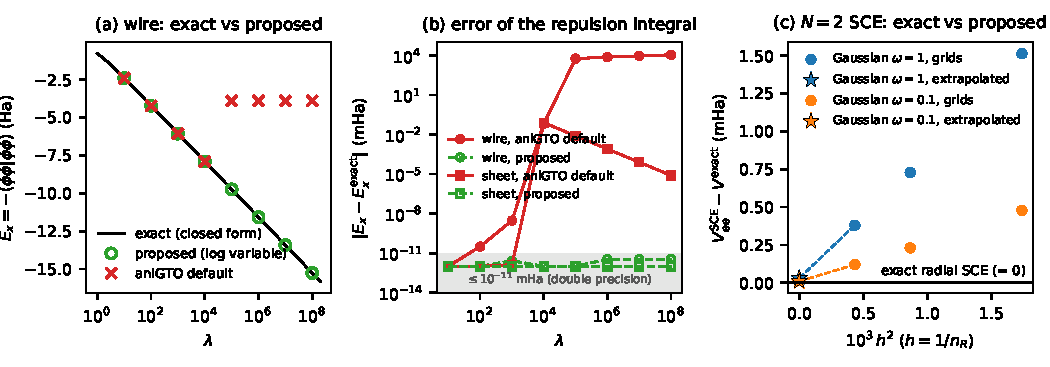
\includegraphics[width=\linewidth]{scan1d2d_dcscan_exact_vs_proposed.pdf}
\caption{(a) Wire self-repulsion versus $\lambda$: closed form (line), $s=\ln u$ quadrature (circles) and aniGTO
  default (crosses), which collapses to $-3.906$~Ha for $\lambda\ge10^5$.  (b) Absolute errors (mHa) for wire and
  sheet; the shaded band is the double-precision limit.  (c) $N=2$ SCE check of the manuscript (not part of
  the ERI method).  Main-text Figure~\href{main.pdf\#figure.caption.5}{1}.}
\label{n:fig}
\end{figure}

%======================================================================================================
\section{The code, verbatim}
\label{n:sec:listings}
The listings below are copied automatically from \texttt{codes/04\_exact\_vs\_proposed.py} at every build
(\texttt{manuscript/make\_eri\_snippets.py}), so they are the code that produced Table~\ref{n:tab}.  The
first two are copied verbatim from aniGTO; only \texttt{IEE\_robust} is new.

\begin{lstlisting}[caption={aniGTO kernel: Gaussian moments (eq~\ref{n:moment}), products of four monomials
  (eq~\ref{n:int2}) and the closed-form $I_k(u^2)$ (eqs~\ref{n:x1}--\ref{n:Ik-closed}).},label=n:code:kernel]
# codes/04_exact_vs_proposed.py (verbatim)

def fact2(n):
    """Calculate the double factorial (n - 1)!! of a non-negative integer 'n'."""
    result = 1
    for i in range(n, 1, -2):
        result *= i
    return result

def integral(a,b):
    r"""this function evaluate an integral like this:
    int_{-\infty}^{+\infty}dx x^a e^{-bx^2}
    """
    if a%2==0.00000000000000000:
        return np.sqrt(np.pi/b)*fact2(a-1)/(2*b)**(a/2)
    else:
        return 0.000000000000000000000

def integral2(alpha,U,a,A,b,B,c,C,d,D):
    """this function evaluates an integral like the one above"""
    N=0.000000000000000000000
    for i in range(a+1):
        for j in range(b+1):
            for k in range(c+1):
                for r in range(d+1):
                    N=N+comb(a,i)*comb(b,j)*comb(c,k)*comb(d,r)*(U-A)**(a-i)*(U-B)**(b-j)*(U-C)**(c-k)*(U-D)**(d-r)*integral(i+j+k+r,alpha)
    return N

def integral3(u2,a,n,A,b,m,B,c,p,C,d,q,D):
    """evaluates the integral over x_1 and x_2 only
    which is the on above"""
    xi=(a+b)*u2/(a+b+u2)
    PAB=(a*A+b*B)/(a+b)
    PCD=(c*C+d*D)/(c+d)
    U=((c+d)*PCD+xi*PAB)/(c+d+xi)
    A1=(A*(a+b+u2)-(a+b)*PAB)/u2
    B1=(B*(a+b+u2)-(a+b)*PAB)/u2
    N=0.000000000000000000000000000000
    for i in range(n+1):
        for j in range(m+1):
            if (i+j)%2==0:
                N=N+comb(n,i)*comb(m,j)*fact2(i+j-1)/(2*a+2*b+2*u2)**((i+j)/2)*((u2)/(a+b+u2))**(n+m-i-j)*np.exp(-(c+d)*xi/(c+d+xi)*(PAB-PCD)**2)*integral2(c+d+xi,U,n-i,A1,m-j,B1,p,C,q,D)
            else:
                N=N+0.0000000000000000000000000000
    return np.sqrt(np.pi/(a+b+u2))*N
\end{lstlisting}

\begin{lstlisting}[caption={aniGTO default: the Boys-type integral in $t$ (eq~\ref{n:eri-t}); baseline of
  Table~\ref{n:tab}.},label=n:code:default]
# codes/04_exact_vs_proposed.py (verbatim)

def integrand2(t, a, l1, A, b, l2, B, c, l3, C, d, l4, D):
    """Define the integrand for numerical integration."""
    ax, ay, az = a
    nx, ny, nz = l1
    Ax, Ay, Az = A
    bx, by, bz = b
    mx, my, mz = l2
    Bx, By, Bz = B
    cx, cy, cz = c
    px, py, pz = l3
    Cx, Cy, Cz = C
    dx, dy, dz = d
    qx, qy, qz = l4
    Dx, Dy, Dz = D
    u2 = t**2 / (1 - t**2)
    return (
        np.power(1 - t**2, -1.50000000000000000000000000000000000000)
        * integral3(u2, ax, nx, Ax, bx, mx, Bx, cx, px, Cx, dx, qx, Dx)
        * integral3(u2, ay, ny, Ay, by, my, By, cy, py, Cy, dy, qy, Dy)
        * integral3(u2, az, nz, Az, bz, mz, Bz, cz, pz, Cz, dz, qz, Dz)
    )

def IEE(a,l1,A,b,l2,B,c,l3,C,d,l4,D):
    ax,ay,az=a
    Ax,Ay,Az=A
    bx,by,bz=b
    Bx,By,Bz=B
    cx,cy,cz=c
    Cx,Cy,Cz=C
    dx,dy,dz=d
    Dx,Dy,Dz,=D
    ExAB=np.exp(-ax*bx*(Ax-Bx)**2/(ax+bx))
    EyAB=np.exp(-ay*by*(Ay-By)**2/(ay+by))
    EzAB=np.exp(-az*bz*(Az-Bz)**2/(az+bz))
    ExCD=np.exp(-cx*dx*(Cx-Dx)**2/(cx+dx))
    EyCD=np.exp(-cy*dy*(Cy-Dy)**2/(cy+dy))
    EzCD=np.exp(-cz*dz*(Cz-Dz)**2/(cz+dz))

    integral,error=quad(integrand2,0.0000000000000,1.00000000000000000000000,(a,l1,A,b,l2,B,c,l3,C,d,l4,D),epsrel =1e-16, epsabs= 1e-16)


    return 2.00000000000000000000000/np.sqrt(np.pi)*ExAB*EyAB*EzAB*ExCD*EyCD*EzCD*integral
\end{lstlisting}

\begin{lstlisting}[caption={\textbf{Proposed}: the same integral in $s=\ln u$ with range, breakpoints and the
  analytic small-$u$ piece (eqs~\ref{n:logvar}--\ref{n:final}).},label=n:code:robust]
# codes/04_exact_vs_proposed.py (verbatim)

def IEE_robust(a, l1, A, b, l2, B, c, l3, C, dd, l4, D):
    """Drop-in replacement for IEE.  Same aniGTO 1-D kernel (integral3), but the Boys-type
    integral is taken in s = ln u instead of t = u / sqrt(1 + u^2):  dt (1 - t^2)^(-3/2) = du, so
        int_0^1 integrand2(t) dt = int ds e^s prod_k integral3(e^{2s}, ...)_k.
    In t the region u^2 ~ exponent ratio sits at 1 - t ~ 1/(2u^2) and is lost to round-off (and 1 - t^2
    underflows to 0) once the ratio exceeds ~1e10; in s it is an ordinary O(1)-wide feature.
    Range: s in [ln sqrt(min exp) - 20, ln sqrt(max exp) + 20], unit breakpoints, plus u0 f(0) for [0, u0]."""
    E = 1.0
    for (p, P), (q, Q) in (((a, A), (b, B)), ((c, C), (dd, D))):
        for k in range(3):
            E *= np.exp(-p[k] * q[k] * (P[k] - Q[k]) ** 2 / (p[k] + q[k]))

    def f(s):
        u2 = np.exp(2.0 * s)
        return np.exp(s) * np.prod([integral3(u2, a[k], l1[k], A[k], b[k], l2[k], B[k], c[k], l3[k], C[k],
                                                     dd[k], l4[k], D[k]) for k in range(3)])
    ex = np.array([a, b, c, dd], dtype=float)
    lo, hi = 0.5 * np.log(ex.min()) - 20.0, 0.5 * np.log(ex.max()) + 20.0
    val, _ = quad(f, lo, hi, points=np.arange(np.floor(lo) + 1.0, hi, 1.0), limit=4000, epsrel=1e-13, epsabs=0.0)
    return 2.0 / np.sqrt(np.pi) * E * (val + f(lo))
\end{lstlisting}

\begin{lstlisting}[caption={Exact test: $E_x=-(\phi\phi|\phi\phi)$ of the wire and sheet (eqs~\ref{n:ex} and
  \ref{n:self}); \texttt{fn} is \texttt{IEE} or \texttt{IEE\_robust}.},label=n:code:test]
# codes/04_exact_vs_proposed.py (verbatim)

def diag_A(family, lam):
    return (lam ** 2, lam ** 2, 1.0) if family == 'wire' else (1.0, 1.0, lam ** 2)

def self_repulsion(family, lam, fn):
    Adiag = np.array(diag_A(family, lam))
    a = tuple(Adiag / 2.0)
    O, L = (0.0, 0.0, 0.0), (0, 0, 0)
    norm4 = np.prod(Adiag) / np.pi ** 3
    return -norm4 * fn(a, L, O, a, L, O, a, L, O, a, L, O)
\end{lstlisting}

\noindent Usage, e.g.\ the wire at $\lambda=10^8$ (exponent ratio $10^{16}$):
\begin{lstlisting}[numbers=none,caption={}]
ex = self_repulsion('wire', 1e8, IEE_robust)   # -15.250628199 Ha, closed form eq A11
ex = self_repulsion('wire', 1e8, IEE)          # -3.906470883 Ha: the default fails
\end{lstlisting}

%======================================================================================================
\section{Equation map: what was solved and where it is in the code}
\label{n:sec:map}
\begin{table}[H]
\centering
\caption{Equations of this note, their place in the manuscript/SI, and the function that implements them.}
\label{n:tab:map}
\small
\begin{tabular}{@{}p{4.3cm}p{3.1cm}p{3.2cm}p{4.5cm}@{}}
\toprule
Step & This note & Manuscript / SI & Code \\
\midrule
Trap Hamiltonian, orbitals & eqs~\ref{n:h}--\ref{n:density} & SI eqs~\href{si.pdf\#equation.1}{S1}--\href{si.pdf\#equation.4}{S4} & analytic; \texttt{TrapS} (03) \\
Density fields $n,\nabla n,\nabla\nabla n,\tau$ & -- & SI eqs~\href{si.pdf\#equation.16}{S16}, \href{si.pdf\#equation.17}{S17} & \texttt{density\_fields} (03) \\
Exact exchange, $N=2$ & eq~\ref{n:ex} & main eq~\href{main.pdf\#equation.9}{A9} & \texttt{self\_repulsion}, \texttt{build\_wire} \\
Gaussian product, moments & eqs~\ref{n:gpt}--\ref{n:int2} & SI eqs~\href{si.pdf\#equation.5}{S5}--\href{si.pdf\#equation.7}{S7} & \texttt{fact2}, \texttt{integral}, \texttt{integral2} \\
Laplace transform, factorization & eqs~\ref{n:coulomb}--\ref{n:Ix} & SI eqs~\href{si.pdf\#equation.8}{S8}--\href{si.pdf\#equation.10}{S10} & \texttt{IEE} (structure) \\
$x_1$ and $x_2$ integrals, closed $I_k$ & eqs~\ref{n:x1}--\ref{n:Ik-closed} & SI eqs~\href{si.pdf\#equation.11}{S11}, \href{si.pdf\#equation.12}{S12} & \texttt{integral3} \\
Boys connection (isotropic) & eqs~\ref{n:iso}, \ref{n:boys} & -- & -- \\
Default Boys-type integral in $t$ & eq~\ref{n:eri-t} & SI eq~\href{si.pdf\#equation.13}{S13} & \texttt{integrand2}, \texttt{IEE} \\
Failure analysis & eqs~\ref{n:loc}, \ref{n:tsing} & main Sec.~\href{main.pdf\#section.3}{3} & -- \\
\textbf{Proposed integral in $s=\ln u$} & eqs~\ref{n:logvar}, \ref{n:range}, \ref{n:final} & main eq~\href{main.pdf\#equation.1}{1} & \texttt{IEE\_robust} \\
Exact test integral & eq~\ref{n:self} & SI eq~\href{si.pdf\#equation.15}{S15}, main eq~\href{main.pdf\#equation.44}{A44} & \texttt{self\_repulsion} \\
Closed forms & -- & main eqs~\href{main.pdf\#equation.10}{A10}, \href{main.pdf\#equation.11}{A11} & \texttt{ex\_exact\_sheet}, \texttt{ex\_exact\_wire} \\
Comparison table, figure & Table~\ref{n:tab}, Fig.~\ref{n:fig} & main Table~\href{main.pdf\#table.4}{4} & \texttt{iee\_rows}, \texttt{make\_table\_and\_figure} \\
\bottomrule
\end{tabular}
\end{table}

%======================================================================================================
\section{Where the codes are: \texttt{SCAN\_1D\_2D/codes/01--09}}
\label{n:sec:codes}
All code is in the folder \texttt{codes/} as nine standalone single-file Python scripts.  Each defines every
function it uses (the aniGTO integrals are copied verbatim) and imports only third-party packages, so one
command reproduces its data, e.g.\ \texttt{cd codes \&\& python3 04\_exact\_vs\_proposed.py}.  Outputs go to
\texttt{codes/results/} (CSV, logs, \LaTeX{} table bodies) and \texttt{codes/figures/}.  None of the scripts
solves a Kohn--Sham or SCF equation (Section~\ref{n:sec:hamiltonian}); PySCF is used only to evaluate libxc
functionals on the given density.

\begin{table}[H]
\centering
\caption{The nine scripts and what they produce.}
\label{n:tab:codes}
\small
\begin{tabular}{@{}p{5.6cm}p{7.6cm}p{2.0cm}@{}}
\toprule
Script & Computes (manuscript item) & Needs \\
\midrule
\texttt{01\_wire\_benchmark.py} & wire reference quadrature of LDA/SCAN/DC-SCAN; SI Tables~\href{si.pdf\#table.1}{S1}--\href{si.pdf\#table.3}{S3}, SI Figure~\href{si.pdf\#figure.caption.3}{S1} & numpy, scipy \\
\texttt{02\_sheet\_benchmark.py} & sheet benchmark; main Table~\href{main.pdf\#table.2}{2}, SI Tables~\href{si.pdf\#table.5}{S5}, \href{si.pdf\#table.6}{S6}, SI Figure~\href{si.pdf\#figure.caption.4}{S2} & numpy, scipy \\
\texttt{03\_anigto\_wire\_libxc.py} & wire with aniGTO ingredients: analytic trap orbital, exact exchange from the aniGTO ERI, density derivatives, libxc functionals; main Table~\href{main.pdf\#table.1}{1}, SI Table~\href{si.pdf\#table.4}{S4} & numpy, scipy, pyscf \\
\textbf{\texttt{04\_exact\_vs\_proposed.py}} & \textbf{this note}: default aniGTO ERI versus the $s=\ln u$ ERI, and the $N=2$ SCE solver; main Table~\href{main.pdf\#table.4}{4}, Figure~\href{main.pdf\#figure.caption.5}{1} & numpy, scipy \\
\texttt{05\_refit\_switch\_scales.py} & PBE base and refit of the activation scales; SI Table~\href{si.pdf\#table.8}{S8} & numpy, scipy \\
\texttt{06\_range\_separation\_q1d\_lda.py} & range separation and the quasi-1D LDA (SI Section~\href{si.pdf\#section.6}{S6}) & numpy, scipy \\
\texttt{07\_q1d\_gga\_profiles.py} & quasi-1D LDA/GGA on seven axial profiles; SI Table~\href{si.pdf\#table.9}{S9} & numpy, scipy \\
\texttt{08\_local\_hybrid\_wires.py} & local hybrids and DC-SCAN on $N=2,4,6$ wires (fixed trap orbitals); SI Table~\href{si.pdf\#table.10}{S10} & numpy, scipy, pyscf \\
\texttt{09\_literature\_validation.py} & sheet-limit construction against Constantin and Kaplan--Wagle--Perdew; main Table~\href{main.pdf\#table.3}{3}, SI Table~\href{si.pdf\#table.7}{S7} & numpy, scipy \\
\bottomrule
\end{tabular}
\end{table}

\noindent The whole pipeline is rerun by \texttt{./refresh\_all.sh}, which also rebuilds the manuscript, the SI
and this note.

\begin{thebibliography}{2}
\bibitem{boys1950} S.~F. Boys, Electronic wave functions. I. A general method of calculation for the
  stationary states of any molecular system, \emph{Proc. R. Soc. London A} \textbf{200}, 542--554 (1950),
  DOI: \href{https://doi.org/10.1098/rspa.1950.0036}{10.1098/rspa.1950.0036}.
\bibitem{anigto} G.~Chirchir, S.~Jana, S.~\'Smiga, An Anisotropic Gaussian Integral Package for
  Quasi-Dimensional Quantum-Chemical Simulations, manuscript in preparation (2026).
\end{thebibliography}

\end{document}
